% !TEX root = ../main.tex
\section{Usability Testing of the Survey}\label{sec:usabilitytestingsurvey}

  The usability of the survey was tested for different purposes. {\it First}, when sending out the survey, there is no much room for changing the layout and content of the survey. When changing the survey during the data collection process, it could introduce bias in the data because the participant could interpret the changed content in different ways. {\it Second}, the survey is in a non-controlled environment, meaning that I have no control of who the participants are and where they are from. It is important to make the layout and the questions as universal an understandable as possible. The questions, the flow, and the graphical elements should be understandable across different countries and cultures. 

  The usability testing is divided in two main parts: usability testing in a controlled environment and usability testing in a uncontrolled environment. Beside the specific usability tests performed, it was also conducted a smaller test only focusing on the icons used in the survey.

    \subsection{Testing the wireframes}


    \subsection{Testing the icons used in the survey}\label{sec:usabilityicontest}
      Legge til resultatene som ble gjort her.

  	\subsection{Testing the application in a controlled environment}
    A usability test in an uncontrolled environment...
    Previous test results....

    The test was conducted with 10 students, 5 boys and 5 girls, from the Norwegian University of Science and Technology. The participants had different background, but the majority had a background in Computer Science.

    To ensure the test was conducted in an environment that is close to how the survey works, they brought their own smartphone and they were not told much about the research. They only got a short introduction to the test that would not impact the results from the test. The participants were told how the test would be performed:

      \begin{enumerate}
        \item The participant were asked to speak loud during the test and tell what they were thinking and reason about their choices.
        \item The participants were told that the test was not testing their ability to finish the test.
        \item The participants were explained that they could quit the test if they felt uncomfortable
      \end{enumerate}

    After giving a introduction to the test, the participant got the URL to the survey and they were asked to start whenever they felt ready. In the list below there is listed comments from the participants that was stated during the test.
        
    {\it "How do I get back if I press a wrong answer?"}\\ 
    One of the persons asked how he could get back to previous question if he selected the wrong answer. He expected a button that could take him back to the previous question.
    
    {\it "Too much icons in the screen showing different screenlocks"}\\ 
    The person did find it confusing with all the icons showing the different screenlocks. The  also found it hard to select the correct screenlock that he used on his smartphone. He commented that this should be solved in a other way that would eliminate the ambiguity and confusing visualization with too many icons. One suggestion was to add a description to each of the icons in a list.
      
    {\it "I need to choose a pattern that is hard to guess for the banking account!"}\\ 
    Most of the participants used more time creating a pattern for a banking account than for the other patterns. Some of them also commented that they did spend more time creating this than the other patterns. It was also noticeable that the participants used more time thinking about this pattern.
    
    {\it "Do I choose the size of my hand based on my gender or is it general?"}\\ 
    Four of the participants was unsure how to categorize the size of their hand. Some of the participants also commented that they selected the size based on their gender or unisex.
      
    {\it "Tody my smartphone would probably be categorized as a medium smartphone"}\\The question is in general subjective, but there is no easy way to ask about the screen size. This question might depend on the persons technical experiences with smartphones. Today, most of the smartphones would be categorized as medium, while older smartphones might would fall into the small category.
      
    {\it "I expected to type the pattern more than once"}\\ 
    One of the participants commented that she expected to be asked to type the pattern more than once. She did not specify if she expected to be prompted with a retype right after creating the pattern or in the end of the survey.
      
    {\it "I do read from left to right, but I do also read lines from top to bottom."}\\ 
    Three of the participants either was unsure what the question asked about or did not understand the icons used. 
      
    {\it "I can't see the question becuase the pattern is too big for my screen"}\\
    One of the participant had a small older iPhone that where the survey rendered poorly because the pattern was too big. 
      
    {\it "The last question about my experience with IT and security took a while to understand."}\\ 
    The question was long and complex. Many of the participants used a long time interpreting the question and some of them asked me during the test if they had understood the question correctly.

    \subsection{Testing the application in a uncontrolled environment}
    Observation of incoming data is not a typical usability test, but is rather a quality check to see whether the collected data is reasonable. When sending out the survey on the internet without being present, it is important to quality check the data to see if it looks like some questions or the graphical elements are ambiguous or hard to understand.The survey was first deployed and distributed to a small group of selected people from Norway (ISO country code 'NO').

    After a day, I looked through the data. One of the observations was that one person had selected a quite rare and small country in Africa with the ISO country code starting with 'N'. It is reasonable that this was a typing error or something wrong with the component used in the question. The component used in the question was a third party dropdown list with a flag icon for each country. I found out that the country component took a long time loading and it appeared that it lagged. A possibility is that the person accidentally had selected the wrong country. The component changed and optimized to avoid this situation by changing the component and removing the icons due to reduce loading time.

    The majority of the people would be from Scandinavia and would have the reading direction form left to right. There was observed that 2 persons out of 25 had other reading and writing directing than left to right. Based on statistics, there should only be persons with reading and writing direction from left to right. One assumption is that the two persons selecting an other reading and directing had interpreted the question wrong. This question should be changed to avoid such situation. 

    Besides looking at the data, I received feedback by email from the selected group of persons.

    {\renewcommand\labelitemi{}
    \begin{itemize}
      \item {\it "The dropdown lagged and I accidently selected the wrong country."}
      \item {\it "I use a 8 digit PIN. Should I select PIN code, password or other?"}
    \end{itemize}}


  	\subsection{Changes to the Survey}

  	Before going live with the survey there was conducted two types of tests providing useful insight of how the users experienced the application. The tests is very important due to the quality of the data collected from the survey. Any ambiguities or errors would could cause bias in the data. After the test I would go through all the feedback and the observed data to make any changes needed in the survey.

    \subsubsection*{1) Country dropdown}
    In both tests there was many participants that unintentionally selected the wrong country because the dropdown component lagged. The component used had a flag attached to the country name that used a lot resources to load, and therefore some user experienced that the component was slow. The component was changed and the flag icons were removed. The changes can be seen in Figure \ref{fig:change-country}.

    \subsubsection*{2) Experience question}
    The question was rather complicated and hard to read. The question was changed from "Do you work with or study/studied IT and/or security full time?" to "Do you have a background in IT/Security?".
      
    \subsubsection*{3) Reading and writing direction}
    The first version of the survey just listed three different icons of arrows indicating the reading and writing direction, but it seemed that people misunderstood the icons in some way. This view was changed by adding a description next to the arrow in order to remove any misinterpretations of the directions. The changes are shown in Figure \ref{fig:change-readwrite}.

    \subsubsection*{4) Adding time used on the creation of patterns}
    It was observed that some of the participants in the usability test in the controlled environment was spending more time creating the pattern for banking account. During the test it was not easy to track the time used on different tasks, but it is possible to track the time used on each pattern in the application to see the diversity between the three types. The observation from the test was that some of the participants took their eyes of the screen thinking harder about the pattern they wanted to create for the bank. In this particular test I was present and could observe such situations, but I will not be able to do this in the application and therefore I added the time used. Such time frame can also be used in the analysis. An example of use could be to pick out dishonest attempts that could cause bias in the data. 
      
    \subsubsection*{5) Selection of screenlock}
    The first version of the view had a list of all the screenlocks that are normally used on a smartphone. The feedback from the tests was that is was confusing to select the correct screenlock for several reasons. {\it First}, some of the participants did not understand all the icons used. {\it Second}, it was observed that some of the user did not interpreted all the alternatives and selected the first fit, but it was sometimes wrong when I stopped the user and asked what they actually used. {\it Third}, it appears that some had a screenlock that could fit into several of the icons, making it hard to pick the correct one. The new version of the view replaced all the icons to a dropdown with alternatives. When the user selects a screenlock, a image or description appears below the dropdown so they could get a extra layer of confirmation that they had selected the correct screenlock. The alternative "PIN" was also changes to "PIN (4-digits)" to be specific and eliminate any ambiguity for those who use more than four digits. The reason for specifically choose four digits is because most users are familiar with this at their bank and smartphones. The changes in this view can be seen in Figure \ref{fig:change-screenlock}.
    
    \subsubsection*{6) Scaling pattern selector for smaller devices}
    The 3 times 3 pattern square was set to a specific size based on the width of the screen, but it seemed that some mobile screen lost some of the height from browser navigation bars. As a consequence, the pattern was laying over the question, making it hard to see which pattern they where creating. There was added a mathematical formula to ensure that the pattern square was scaling properly on any screensize. 
    
    \subsubsection*{7) Changing handsize question}
    Based on feedback in the test in the controlled environment, the participants did not know what to compare their handsize to. They often reasoned different sizes compared to their gender and unisex. It was therefore desirable to explicitly state in the question that the user was selecting their size of their hand based on their gender. The question still remains subjective, but by explicitly stating gender as a standard it will remove some bias. 
    
    \subsubsection*{8) Adding pattern retype}
    During the tests I god feedback that many of the participants expected to be asked to retype their selected patterns right after creating it or in the end of the survey. It is not desirable to ask users to retype their patterns in the end of the survey because users then would feel uncomfortable if they did not remember it. It did not want the users to leave the survey with a bad experience. By stating that the users should remember the patterns in the end of the survey could end up with many user leave the survey because they would feel uncomfortable. Some would might also leave the survey because it would require them to actually do more work than they are willing to do for a survey. I decided to ask the user to retype the pattern right after creating because this is how the process works on Android smartphones. On Android devices, the users types a pattern and are thereafter asked to retype the pattern again to create the pattern for their smartphone. \todo{Visualize process in survey and on Android. The pattern cre. proc.}
    
    \subsubsection*{9) Collecting screen pixels of screen used}
    By observing the participants in the first test, I recorded my opinion of their screen size as well as their own choices. About 70\% of their choices matched my own opinion of the screen size. Since this question is a subjective meaning of the person answering, I added an extra layer of information by saving the pixels width and hight of the mobile device. One problem with pixels size of a mobile screen is that they do not match the physical size of the screen. The pixels could still provide information to actually categorize the correct size by comparing the OS and pixels.

    \begin{figure}[H]
      \centering
      \subfigure[Old view]{
        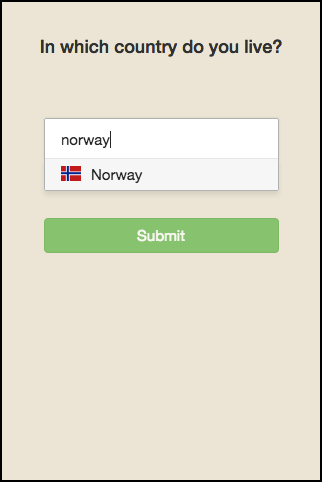
\includegraphics[scale=0.34]{pics/survey/country-old}
      }
      \subfigure[Final view after changes]{
        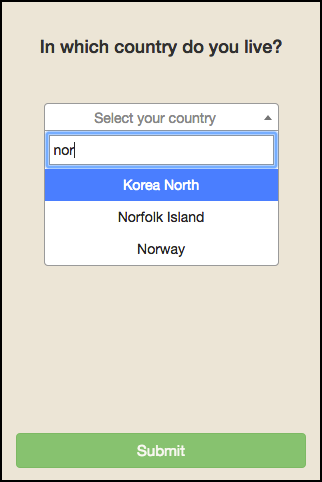
\includegraphics[scale=0.34]{pics/survey/country2}
      }
      \caption{Changes in country selection view}
      \label{fig:change-country}
    \end{figure}

    \begin{figure}[H]
      \centering
      \subfigure[Old view]{
        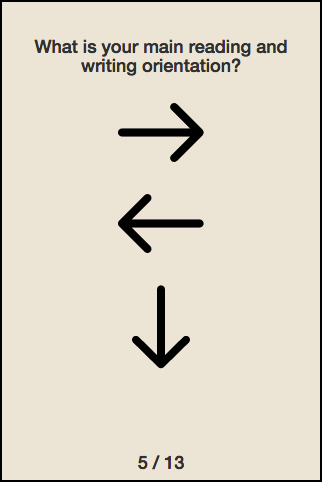
\includegraphics[scale=0.34]{pics/survey/reading-old}
      }
      \subfigure[Final view after changes]{
        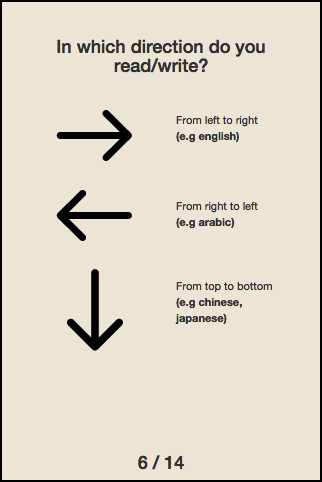
\includegraphics[scale=0.34]{pics/survey/reading}
      }
      \caption{Changes in reading/writing direction view}
      \label{fig:change-readwrite}
    \end{figure}

    \begin{figure}[H]
      \centering
      \subfigure[Old view]{
        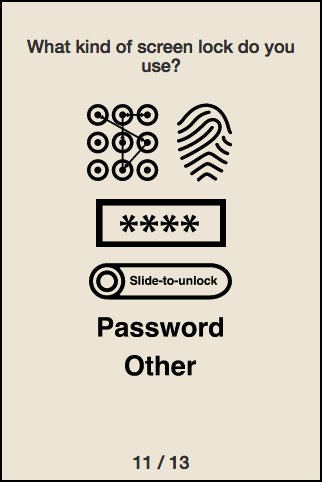
\includegraphics[scale=0.34]{pics/survey/screenlock-old}
      }
      \subfigure[Final view after changes]{
        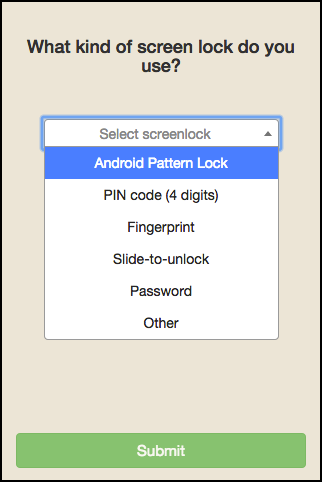
\includegraphics[scale=0.34]{pics/survey/screenlock2}
      }
      \caption{Changes in screenlock selection view}
      \label{fig:change-screenlock}
    \end{figure}

\section{Ethical Considerations}\label{sec:ethics}
    
    - Veileder har vurdert forskningen
    - Kontaktpunktet på NTNU til nsd har godkjent forskningen. Var ikke merket som meldepliktig.

    My research is done by collecting demographics and personal data, as well as asking the respondents to enter three selected patterns. Before doing research it is important to look into the ethical aspects to see if the data collected, is legal and protect the personal data being anonymous.

    Before the questionnaire starts, the respondents are informed about the purpose of the research and how their contributed data will be used. Respondents also must be informed that they have the right not to participate. The questionnaire should be entirely anonymous, and their identity and location should not be possible to track back to the respondent.

    The demographic information collected do not provide any information that make it possible to track the data back to the respondent. It is still needed to apply for an allowance to conduct this research because of collecting personal information. It is not desired to conduct unethical research. This will further be described in the next Chapter for future work.


% -  --> Changed third party component
% -  --> Changes question
% -  --> Added description
% - 
% -  --> Changed to dropdown list
% -  --> 6 different orders.
% - 
% - Question about handsize --> Based on gender
% - Pattern retype --> same process as android
% - Screensize